As always, there are problems with any project. In this project there were problems too.\newline The main problems was to implement the code and working properly.\newline First problem was to how implement graphic in website, but it is easy to solve, but sometimes i had problems with css files, where i saved this and nothing happens. \ref{fig:Css} \newline \newline
Secondly my ArduCam ESP8266-12E WiFi IoT didn't work i didn't know why, so i changed to ethernet shield. Then Ethernet shields need to use some of pins to work properly. The Ethernet shield uses digital pins 11, 12, 13, 10, and 4 for SPI communication, so i couldn't connect my lcddisplay and other stuff: rtc, buttons. Even simple program like "Hello world" didn't want display on lcd. When i changed to analog my program didn't want calculate, so i just removed lcd and other stuff to make project easier. \ref{fig:Esbp} \newline \newline \newline
To create server was a problem too. Probably the problem was in library i used which is ethernet.h then i changed it to ethernet2.h, and i had server but it didn't send data to database I didn't figure out why. \ref{fig:Server}\newline \newline
\begin{figure}[!b]
	\centering
	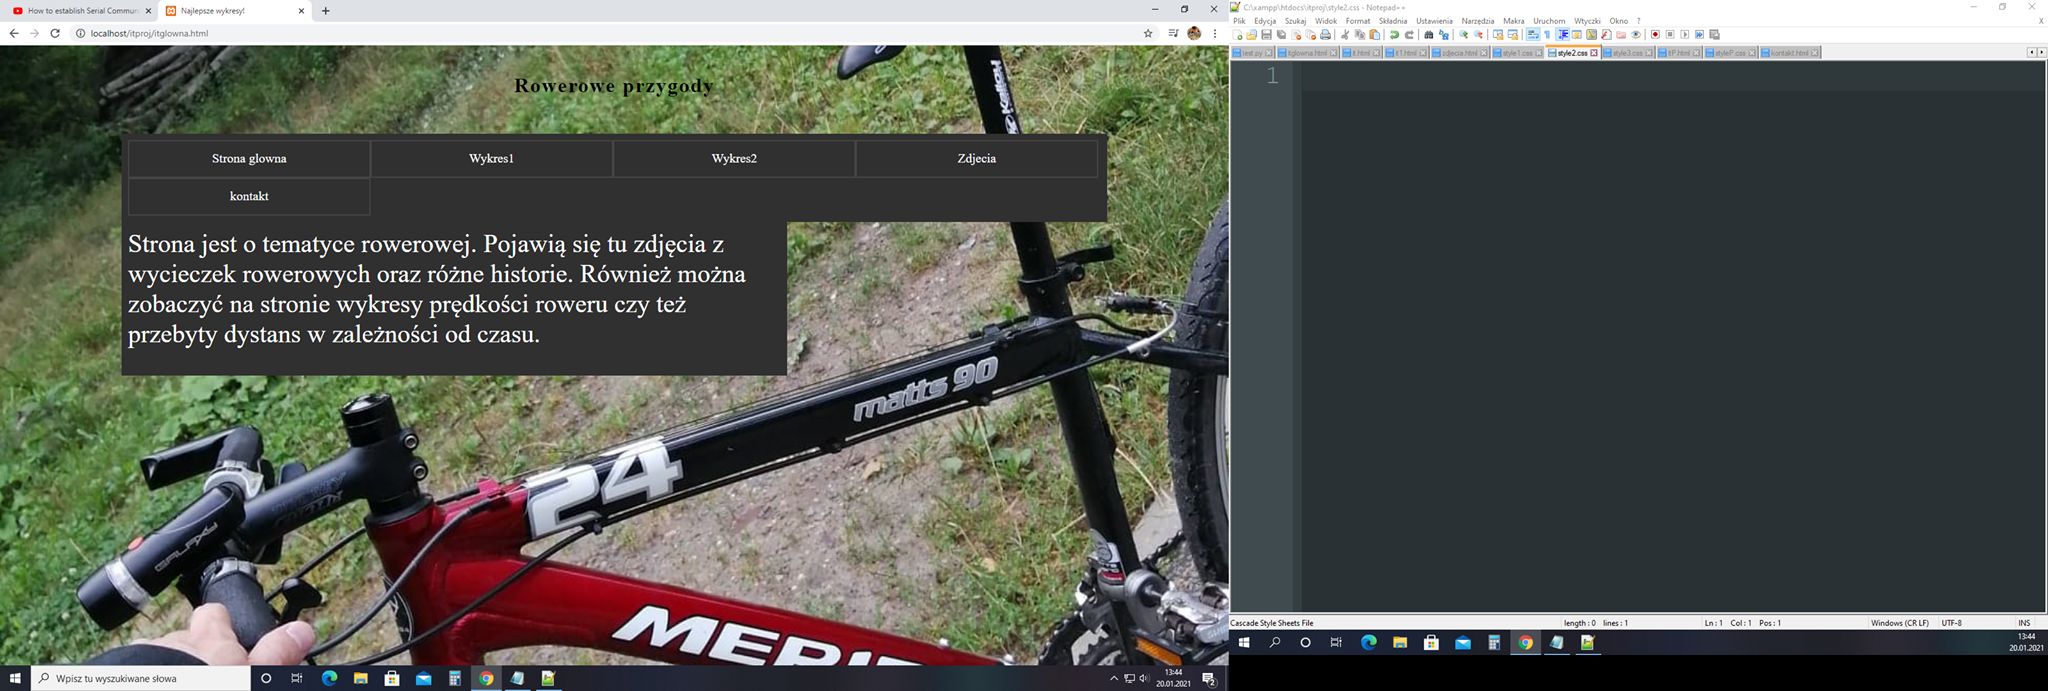
\includegraphics[width=5.0in]{css.png}
	\caption{Css.\label{fig:Css}}
\end{figure}

\begin{figure}[!b]
	\centering
	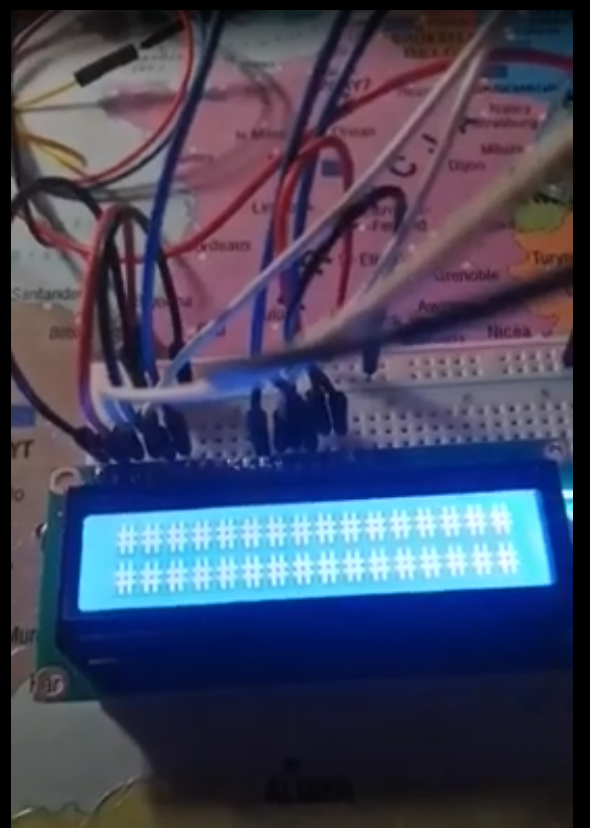
\includegraphics[width=2.7in]{esbp.png}
	\caption{Ethernet Shield pins problem.\label{fig:Esbp}}
\end{figure}

\begin{figure}[!b]
	\centering
	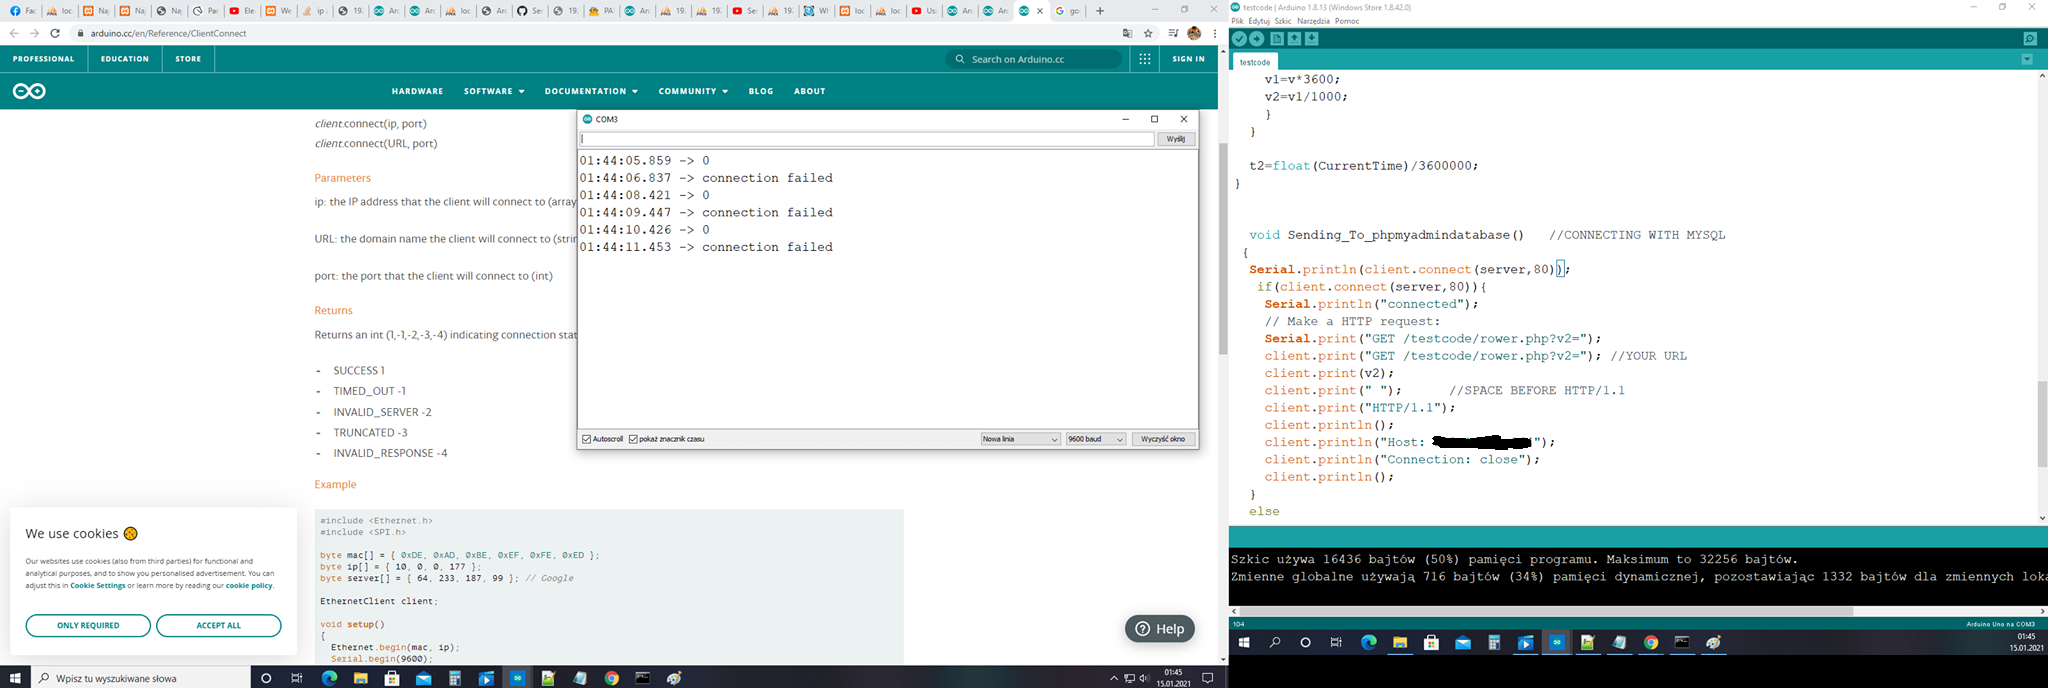
\includegraphics[width=5.0in]{server.png}
	\caption{Server problem.\label{fig:Server}}
\end{figure}